\section{Conceptual Differences from HomeOS}                                                           
\label{sec:homeosdiff}
As we were developing our system, several key changes from the original HomeOS
system were made which were either necessary or determined to be advantageous.
As a result of these differences, we are diverging from HomeOS. As we continue
with the development process, we expect to be significantly different from
HomeOS in the future.  We discuss the key changes in more detail below.
\subsection{Architectural Differences}
\label{sec:archdiff} 
\begin{figure}[tbh]                                                              
    \centering                                                                   
    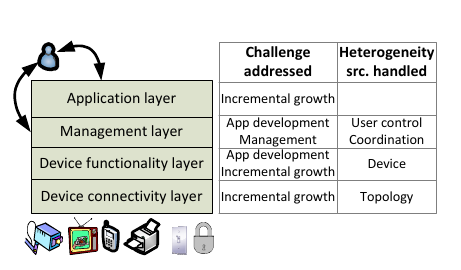
\includegraphics[width=1.0\columnwidth]{figs/homeosOrig.png}                     
    \caption{HomeOS Architecture from~\cite{homeOS}}                                 
    \label{Fig:homeosarch}                                                           
\end{figure}                                                                     
Figure~\ref{Fig:homeosarch} gives an overview of the original HomeOS
architecture taken from the HomeOS paper~\cite{homeOS}.
In the original HomeOS, the architecture of the system has been divided into 
stacked layers, with the application layer at the top. We decided that viewing
applications as components similar to devices and drivers was more intuitive.
This leads us to consider applications at the same level as the devices and
drivers, rather than a layer that sits on top of the management layer. This
leads the Management Component to play a more central and critical role.

HomeOS considers devices and protocols to fit under the same abstraction.
However, we view them as separate entities. We felt this was more intuitive and
might be more advantageous in the future.

Due to limitations with Java, all communication between components has to go
through the Management Component. This was a necessary change. This change has 
been discussed in more detail in the Section~\ref{sec:challenges}.
\subsection{Implementation Differences}
\label{sec:impldiff} 
One of the main differences between the original HomeOS system and our system is
that our system is written in Java rather than C\#. We chose to use Java to try
to maximize the cross-platform capabilities, as well as pull from a larger pool
of developers. We also strived to use only open source libraries to also improve
cross-platform support and encourage community-based development.

While the module access control, discussed in more detail in
Section~\ref{sec:module_access}, closely resembles the access control system
used by HomeOS, the core access control system is of our own design, discussed
in more detail in Section~\ref{sec:core_access}. In addition, while HomeOS used
datalog, we are using database tables to mimic the functionality of datalog.

We felt it was important to provide a flexible data backend and not tie our
system to one particular data storage system. The data backend must provide
certain functionality, but the actual implementation and storage format is left 
to the developer.
